% Drawing 142/02-13 -- folder 142, batch 02, archive page 39 (PDF page 40).
% Transcription: sphère : pôles $P^{+}$, $P^{-}$ ; autour des trois points marqués, les petits cercles $R_i^{\pm}$ avec les arcs $a_i^{\pm}$ ; les méridiens $\tilde d_i^{\pm}$ et $\tilde d_i'^{\pm}$ ($i = 0, 1, \infty$) descendant des pôles vers les $R$, en trait plein ou pointillé selon qu'ils sont vus ou cachés.
% Kind: sphere with poles, meridians and small circles. Method 2 (schematic redraw from the facsimile). Status: partial.
% Notes: Crop widened to the right so that the whole sphere is in it (the earlier crop cut the circle round infinity). Pencil outer outline; P^+ and P^-; the three small circles round the marked points (left R_1^-, R_1^+, a_1^+-; middle R_0^+, R_0^-, a_0^+-; right R_infty^-, R_infty^+, a_infty^+-), each with its dot, its two vertices at its left and right ends and its two arcs; the twelve meridians tilde d_i^+-, tilde d_i'^+- from the poles to these vertices, each with its arrow into the vertex and all those of a pole leaving the same pole point: tilde d_0'^+ and tilde d_0'^- dashed, the others solid; the dashed equator (from R_1^- round the left edge to R_0^+, from R_1^+ to R_infty^-, and from R_0^- towards the circle round infinity). Still differs: the arrowheads on the small circles are not drawn; the inked front outline is drawn as the outer meridians tilde d_1'^+ and tilde d_infty^+ only; which inner meridians are dashed is a reading of faint strokes; the label R_infty^+ is cut by the edge of the page, and the blot on tilde d_1^+ near the top is not drawn. Nothing is struck. The legend (VII?) at the bottom right is text. Redrawn 2026-11-09 (issue 128): to check again.
% Coordinates: 1 unit = 1 mm = 1/100 of the crop width (bbox in page fractions: [0.12, 0.455, 0.39, 0.665]).
% Redrawn by Claude (claude-opus-5-5), issue #73, 2026-11-09; not checked by a human; not compiled (no TeX in the session).
% Rights: reproduces part of the work -- behind RENDER_TRANSCRIPTS, never published by itself.
\documentclass[tikz,border=3pt]{standalone}
\usepackage{amsmath,amssymb}
\usetikzlibrary{patterns,arrows.meta}
\tikzset{pencil/.style={black!45}, struck/.style={black!35}, mark/.style={circle,draw,inner sep=1.3pt}, pt/.style={circle,fill,inner sep=0.9pt}, opt/.style={circle,draw,fill=white,inner sep=1.1pt}}
\begin{document}
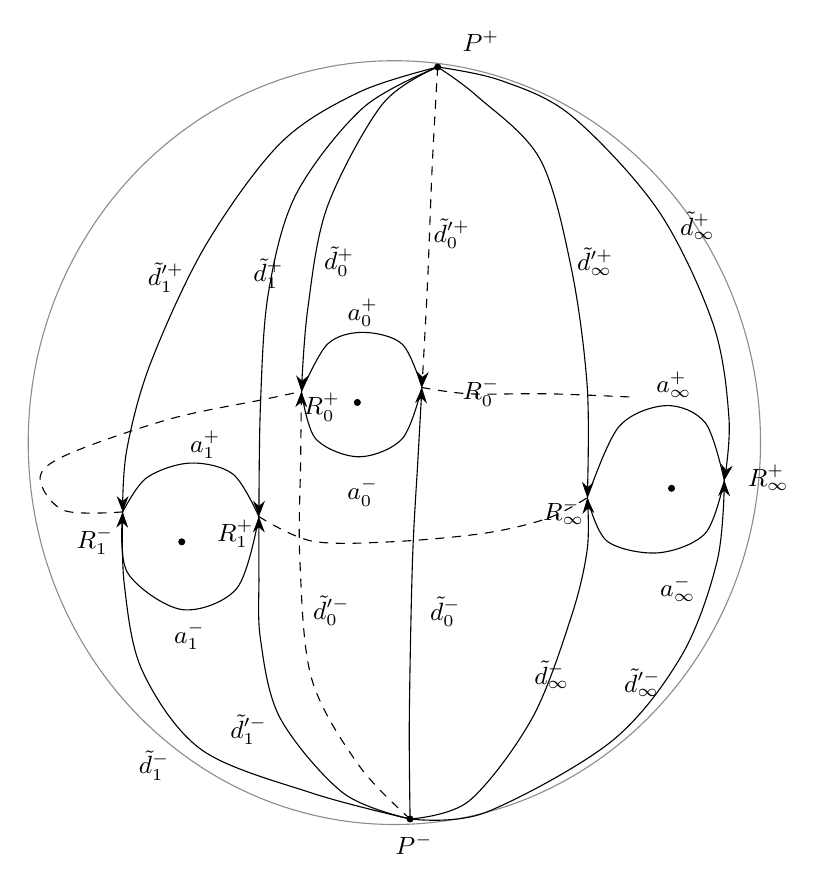
\begin{tikzpicture}[x=1mm,y=1mm,line cap=round,line join=round,font=\scriptsize]
\draw[pencil] (50.5,-55) ellipse[x radius=46.5, y radius=48.5];
\node[pt] at (56,-7.3) {};
\node[pt] at (52.5,-102.8) {};
\node[pt] at (23.5,-67.6) {};
\node[pt] at (45.8,-49.9) {};
\node[pt] at (85.7,-60.8) {};
\draw plot[smooth, tension=0.55] coordinates {(16,-63.8) (19,-59.5) (24.5,-57.6) (30,-59) (33.3,-64.4)};
\draw plot[smooth, tension=0.55] coordinates {(16,-63.8) (16.6,-71.5) (23.5,-76.2) (30.5,-73.5) (33.3,-64.4)};
\draw plot[smooth, tension=0.55] coordinates {(38.7,-48.5) (42,-42.5) (46.5,-41) (51.5,-42.5) (54,-48)};
\draw plot[smooth, tension=0.55] coordinates {(38.7,-48.5) (40.5,-54.5) (46,-56.8) (51.5,-54.5) (54,-48)};
\draw plot[smooth, tension=0.55] coordinates {(75,-62) (79,-53) (85,-50.3) (90,-52.5) (92.4,-59.8)};
\draw plot[smooth, tension=0.55] coordinates {(75,-62) (77.5,-67.5) (84,-69) (90,-66.5) (92.4,-59.8)};
\draw[-{Stealth[length=2mm]}] plot[smooth, tension=0.55] coordinates {(56,-7.3) (46,-10.5) (36,-17) (26.5,-30) (19.5,-45) (16.5,-56) (16,-63.8)};
\draw[-{Stealth[length=2mm]}] plot[smooth, tension=0.55] coordinates {(56,-7.3) (46.5,-12.5) (38,-23.5) (34.5,-36) (33.5,-50) (33.3,-64.4)};
\draw[-{Stealth[length=2mm]}] plot[smooth, tension=0.55] coordinates {(56,-7.3) (49,-12) (42,-25) (39.5,-38) (38.7,-48.5)};
\draw[dashed,-{Stealth[length=2mm]}] plot[smooth, tension=0.55] coordinates {(56,-7.3) (55.3,-20) (54.7,-35) (54,-48)};
\draw[-{Stealth[length=2mm]}] plot[smooth, tension=0.55] coordinates {(56,-7.3) (61,-11) (69,-19) (73,-33) (75,-48) (75,-62)};
\draw[-{Stealth[length=2mm]}] plot[smooth, tension=0.55] coordinates {(56,-7.3) (64,-9) (73,-13.5) (84,-25.5) (91,-40) (93,-52) (92.4,-59.8)};
\draw[-{Stealth[length=2mm]}] plot[smooth, tension=0.55] coordinates {(52.5,-102.8) (40,-99.5) (26,-94) (18.5,-84) (16.2,-73) (16,-63.8)};
\draw[-{Stealth[length=2mm]}] plot[smooth, tension=0.55] coordinates {(52.5,-102.8) (44,-99.5) (36,-90) (33.5,-80) (33.3,-72) (33.3,-64.4)};
\draw[dashed,-{Stealth[length=2mm]}] plot[smooth, tension=0.55] coordinates {(52.5,-102.8) (46,-96) (40,-85) (38.5,-70) (38.6,-57) (38.7,-48.5)};
\draw[-{Stealth[length=2mm]}] plot[smooth, tension=0.55] coordinates {(52.5,-102.8) (52.4,-90) (52.8,-70) (53.5,-57) (54,-48)};
\draw[-{Stealth[length=2mm]}] plot[smooth, tension=0.55] coordinates {(52.5,-102.8) (60,-100.5) (68,-90) (73,-77) (75,-68.5) (75,-62)};
\draw[-{Stealth[length=2mm]}] plot[smooth, tension=0.55] coordinates {(52.5,-102.8) (62,-102) (78,-93) (87,-82) (91.5,-70) (92.4,-59.8)};
\draw[dashed] plot[smooth, tension=0.55] coordinates {(16,-63.8) (8.5,-63.6) (5.5,-59.5) (9,-56.5) (22,-52) (34,-49.5) (38.7,-48.5)};
\draw[dashed] plot[smooth, tension=0.55] coordinates {(54,-48) (60,-48.8) (70,-48.8) (80.3,-49.2)};
\draw[dashed] plot[smooth, tension=0.55] coordinates {(33.3,-64.4) (40,-67.5) (50,-67.6) (62,-66.5) (70,-64.6) (75,-62)};
\node[inner sep=1pt] at (61.5,-4) {\small $P^{+}$};
\node[inner sep=1pt] at (53,-106) {\small $P^{-}$};
\node[inner sep=1pt] at (21.5,-34) {\small $\tilde d_1'^{+}$};
\node[inner sep=1pt] at (34.5,-33.5) {\small $\tilde d_1^{+}$};
\node[inner sep=1pt] at (43.5,-32) {\small $\tilde d_0^{+}$};
\node[inner sep=1pt] at (57.8,-28.5) {\small $\tilde d_0'^{+}$};
\node[inner sep=1pt] at (76,-32) {\small $\tilde d_\infty'^{+}$};
\node[inner sep=1pt] at (89,-27.5) {\small $\tilde d_\infty^{+}$};
\node[inner sep=1pt] at (20,-96) {\small $\tilde d_1^{-}$};
\node[inner sep=1pt] at (32,-91.5) {\small $\tilde d_1'^{-}$};
\node[inner sep=1pt] at (42.5,-76.4) {\small $\tilde d_0'^{-}$};
\node[inner sep=1pt] at (57,-76.5) {\small $\tilde d_0^{-}$};
\node[inner sep=1pt] at (70.5,-84.5) {\small $\tilde d_\infty^{-}$};
\node[inner sep=1pt] at (82,-85.5) {\small $\tilde d_\infty'^{-}$};
\node[inner sep=1pt] at (12.5,-67.5) {\small $R_1^{-}$};
\node[inner sep=1pt] at (30.3,-66.6) {\small $R_1^{+}$};
\node[inner sep=1pt] at (26.5,-55.3) {\small $a_1^{+}$};
\node[inner sep=1pt] at (24.5,-79.5) {\small $a_1^{-}$};
\node[inner sep=1pt] at (41.3,-50.5) {\small $R_0^{+}$};
\node[inner sep=1pt] at (61.5,-48.6) {\small $R_0^{-}$};
\node[inner sep=1pt] at (46.5,-38.5) {\small $a_0^{+}$};
\node[inner sep=1pt] at (46.5,-61.3) {\small $a_0^{-}$};
\node[inner sep=1pt] at (72,-63.8) {\small $R_\infty^{-}$};
\node[inner sep=1pt] at (98,-59.5) {\small $R_\infty^{+}$};
\node[inner sep=1pt] at (86,-47.6) {\small $a_\infty^{+}$};
\node[inner sep=1pt] at (86.5,-73.5) {\small $a_\infty^{-}$};
\end{tikzpicture}
\end{document}
